\chapter{Ergebnis}

Die in der Studie getesteten Personen waren Studenten der TU München und wiesen folgende Merkmale auf:

    \begin{itemize}
        \item 35,9 Prozent von ihnen waren weiblich 
        \item die Probandinnen und Probanden kamen mit 66,7 Prozent überwiegend aus Bayern
        \item die Studenten waren im Mittel im 3,85 Fachsemester
    \end{itemize}

 Um die Forschungsfrage (1) zu untersuchen, wurden die Gruppen mit Hilfe einer Varianzanalyse auf folgende Werte untersucht:
    \begin{itemize}
        \item Fixationen auf dem Bild 
        \item Fixationen auf dem Text
        \item Dauer des ersten Durchgangs
        \item Dauer des zweiten Durchgangs 
    \end{itemize}

\begin{figure}[H]
\noindent\hspace{0.5mm}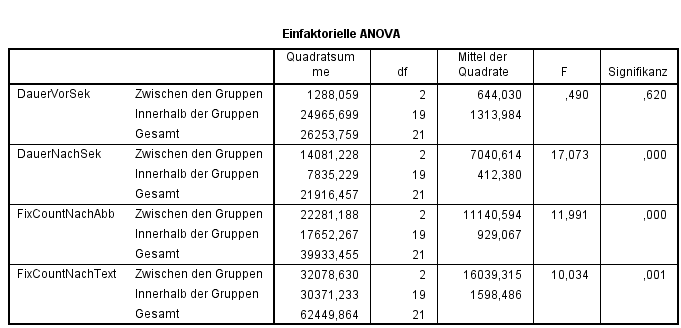
\includegraphics[width=15cm]{./Ressourcen/Gruppenunterscheidung.png}
\caption{Gruppenvarianz, Lorenz Müller}
\end{figure}

Widmet man sich der zweiten Forschungsfrage, kommt man zu folgenden Ergebnissen:
Alle Studenten erzielten im Schnitt 6,03 Punkte. 
Die jeweiligen Gruppen erzielten für die Bearbeitung aller Aufgaben im Durchschnitt folgende Punkte:

\begin{table}[H]
\hspace{-5pt}
\begin{tabularx}{\textwidth + 5pt}{| @{\hspace{3pt}} M || @{\hspace{3pt}} M  | @{\hspace{3pt}} M | @{\hspace{3pt}} M |}
\hline
\textbf{ } & \textbf{Typ Unsicher (Gr1.)} & \textbf{Typ Problemlöser (Gr2.)} & \textbf{Typ Textuell (Gr3.)}\\
\hline
\hline
Punkte        & 6,17 & 5,5 & 6,3\\
\hline
\end{tabularx}
\caption{Mittelwert der Punkte der Probandengruppen}
\end{table}


Bei der Untersuchung nach signifikanten Unterschieden, wurde
die Varianzanalyse über die Gesamtpunktzahl gestellt, welche folgende Ergebnisse herbrachte:

\begin{figure}[H]
\noindent\hspace{0.5mm}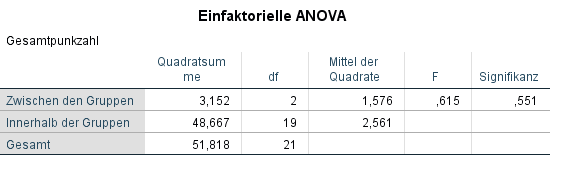
\includegraphics[width=15cm]{./Ressourcen/Punktevarianz.png}
\caption{Punktevarianz, Lorenz Müller}
\end{figure}

Wendet man sich nun der dritten Forschungsfrage, dem Einfluss der gewählten Bilder in der Betrachtung der Antworten aller Pobandinnen und Probanden zu, ergibt sich folgendes Bild: 


\begin{table}[H]
\hspace{-5pt}
\begin{tabularx}{\textwidth + 5pt}{| @{\hspace{3pt}} M || @{\hspace{3pt}} M  | @{\hspace{3pt}} M | @{\hspace{3pt}} M |}
\hline
\textbf{Aufgabe} & \textbf{Radfahrerin 1 (ARad.)} & \textbf{Radfahrerin 2 (ARad.)} & \textbf{Rennfahrer (ARen.)} \\
\hline
\hline
Prozent richtig beantwortet       & 97,5 & 17,9 & 76,9 \\
\hline
\end{tabularx}
\caption{Mittelwert der Wertungspunkte pro Aufgabe 1}
\end{table}

\begin{table}[H]
\hspace{-5pt}
\begin{tabularx}{\textwidth + 5pt}{| @{\hspace{3pt}} M | @{\hspace{3pt}} M  | @{\hspace{3pt}} M | @{\hspace{3pt}} M |}
\hline
\textbf{Zufall} & \textbf{Berg 1 (ABerg.)} & \textbf{Berg 2 (ABerg.)} & \textbf{Autofahren (AAut.)}\\
\hline
\hline
    51,3 & 76,9 & 74,3 &  94,9\\
\hline
\end{tabularx}
\caption{Mittelwert der Wertungspunkte pro Aufgabe 2}
\end{table}

Im Schnitt wurden somit die jeweiligen Bildtypen mit folgenden Prozentwerten richtig beantwortet. 

\begin{table}[H]
\hspace{-5pt}
\begin{tabularx}{\textwidth + 5pt}{| @{\hspace{3pt}} M || @{\hspace{3pt}} M  | @{\hspace{3pt}} M | @{\hspace{3pt}} M |}
\hline
\textbf{Aufgabentyp} & \textbf{dekorativ} & \textbf{essenziell} \\
\hline
\hline
Prozent richtig beantwortet       & 66,7 & 74,3 \\
\hline
\end{tabularx}
\caption{Mittelwert dekorativ bzw. essenziell}
\end{table}

Bei der Untersuchung nach signifikanten Unterschieden entsteht folgende Varianzanalyse:


\begin{figure}[H]
\noindent\hspace{0.5mm}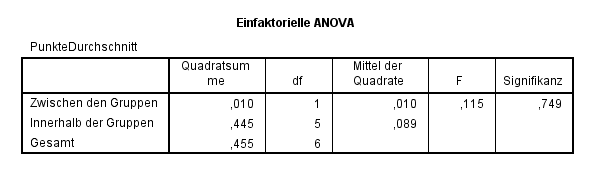
\includegraphics[width=15cm]{./Ressourcen/Aufgabenuntescheidung.png}
\caption{Punktevarianz, Lorenz Müller}
\end{figure}




Widmet man sich nun der vierten Forschungsfrage (Auswirkungen von bestimmten Aufgabentypen auf die Probandengruppen), lassen sich folgenden Feststellungen treffen.
Bei der Auswertung der einzelnen Gruppen wurden die Ergebnisse fett markiert, welche sich um mehr als 20 Prozent vom Wert der Allgemeinheit unterschieden:

\section*{Problemlöser}
\begin{table}[H]
\hspace{-5pt}
\begin{tabularx}{\textwidth + 5pt}{| @{\hspace{3pt}} M || @{\hspace{3pt}} M  | @{\hspace{3pt}} M | @{\hspace{3pt}} M |}
\hline
\textbf{Aufgabe} & \textbf{Radfahrerin 1 (ARad.)} & \textbf{Radfahrerin 2 (ARad.)} & \textbf{Rennfahrer (ARen.)} \\
\hline
\hline
Prozent richtig beantwortet       & 100 & 10 & 90 \\
\hline
\end{tabularx}
\caption{Typ Problemlöser bei den unteschiedlichen Aufgabenstellungen 1}
\end{table}


\begin{table}[H]
\hspace{-5pt}
\begin{tabularx}{\textwidth + 5pt}{| @{\hspace{3pt}} M | @{\hspace{3pt}} M  | @{\hspace{3pt}} M | @{\hspace{3pt}} M |}
\hline
\textbf{Zufall (AZuf.)} & \textbf{Berg 1 (ABerg.)} & \textbf{Berg 2 (ABerg.)} & \textbf{Autofahren (AAut.)}\\
\hline
\hline
    40 & 60 & 70 &  \textbf{50}\\
\hline
\end{tabularx}
\caption{Typ Problemlöser bei den unteschiedlichen Aufgabenstellungen 2}
\end{table}

\section*{Unsichere}
\begin{table}[H]
\hspace{-5pt}
\begin{tabularx}{\textwidth + 5pt}{| @{\hspace{3pt}} M || @{\hspace{3pt}} M  | @{\hspace{3pt}} M | @{\hspace{3pt}} M |}
\hline
\textbf{Aufgabe} & \textbf{Radfahrerin 1 (ARad.)} & \textbf{Radfahrerin 2 (ARad.)} & \textbf{Rennfahrer (ARen.)} \\
\hline
\hline
Prozent richtig beantwortet       & 83 & 17 & 67 \\
\hline
\end{tabularx}
\caption{Typ Unsicher bei den unteschiedlichen Aufgabenstellungen 1}
\end{table}

\begin{table}[H]
\hspace{-5pt}
\begin{tabularx}{\textwidth + 5pt}{| @{\hspace{3pt}} M | @{\hspace{3pt}} M  | @{\hspace{3pt}} M | @{\hspace{3pt}} M |}
\hline
\textbf{Zufall (AZuf.)} & \textbf{Berg 1 (ABerg.)} & \textbf{Berg 2 (ABerg.)} & \textbf{Autofahren (AAut.)}\\
\hline
\hline
    \textbf{83} & 83 & 67 &  100\\
\hline
\end{tabularx}
\caption{Typ Unsicher bei den unteschiedlichen Aufgabenstellungen 2}
\end{table}

\section*{Textuelle}
\begin{table}[H]
\hspace{-5pt}
\begin{tabularx}{\textwidth + 5pt}{| @{\hspace{3pt}} M || @{\hspace{3pt}} M  | @{\hspace{3pt}} M | @{\hspace{3pt}} M |}
\hline
\textbf{Aufgabe} & \textbf{Radfahrerin 1 (ARad.)} & \textbf{Radfahrerin 2 (ARad.)} & \textbf{Rennfahrer (ARen.)} \\
\hline
\hline
Prozent richtig beantwortet       & 100 & 17 & \textbf{100} \\
\hline
\end{tabularx}
\caption{Typ Textuell bei den unteschiedlichen Aufgabenstellungen 1}
\end{table}


\begin{table}[H]
\hspace{-5pt}
\begin{tabularx}{\textwidth + 5pt}{| @{\hspace{3pt}} M | @{\hspace{3pt}} M  | @{\hspace{3pt}} M | @{\hspace{3pt}} M |}
\hline
\textbf{Zufall (AZuf.)} & \textbf{Berg 1 (ABerg.)} & \textbf{Berg 2 (ABerg.)} & \textbf{Autofahren (AAut.)}\\
\hline
\hline
    67 & 67 & 67 &  83\\
\hline
\end{tabularx}
\caption{Typ Textuell bei den unteschiedlichen Aufgabenstellungen 2}
\end{table}

Mit Hilfe der Varianzanalyse wurde untersucht, ob sich auffällige Ergebnisse signifikant von der Allgemeinheit unterscheiden: 

\begin{itemize}
    \item Autofahrt wurde von dem (Gr1.) mit nur 50 Prozent richtig gelöst. (Allgemeinheit 94,9 Prozent) ($\alpha$ = 0,243 F = 1,407)
    \item Zufall wurde von dem (Gr2.) mit 83,3 Prozent richtig gelöst. (Allgemeinheit 0,513) ($\alpha$ = 0,152 F = 2,135)
    \item Rennfahrer wurde von (Gr3.) von allen Versuchsteilnehmern richtig gelöst. (Allgemeinheit 0,769) ($\alpha$ = 0,092 F = 2,990)
\end{itemize}

Betrachtet man noch abschließend, wie sich die unterschiedlichen Lerntypen unter Einfluss Bildtypen verhalten haben, so ergibt sich folgendes Bild.

\begin{table}[H]
\hspace{-5pt}
\begin{tabularx}{\textwidth + 5pt}{| @{\hspace{3pt}} M | @{\hspace{3pt}} M  | @{\hspace{3pt}} M | @{\hspace{3pt}} M |}
\hline
\textbf{Lerntyp} & \textbf{Unsicher} & \textbf{Problemlöser} & \textbf{Textuell}\\
\hline
\hline
    dekorativ & 62,5 & 60 &  62,5\\
\hline
    essenziell & 83,3 & 60,0 &  83,3\\
\hline
\end{tabularx}
\caption{dekorative und essenzielle Bildtypen mit Berücksichtigung der Lerntypen}
\end{table}

Mit der Varianzanalyse:  

\begin{figure}[H]
\noindent\hspace{0.5mm}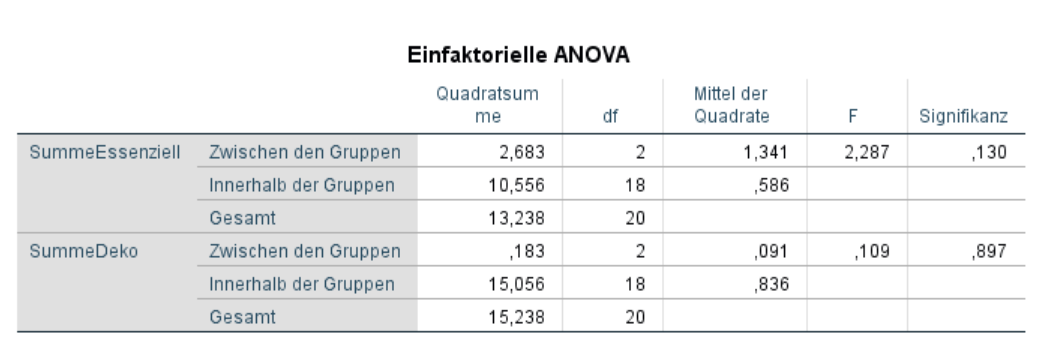
\includegraphics[width=15cm]{./Ressourcen/DekoEssGruppen.png}
\caption{dekorative und essenzielle Bildtypen mit Berücksichtigung der Lerntypen, Lorenz Müller}
\end{figure}

